\documentclass{pre-tfg}

%\showhelp  % comenta o borra para eliminar ayudas

\title{Sistema de Vigilancia Adaptativo basado en la Coordinación de UAVs en Entornos Afectados por Catástrofes}
\author{Juan Manuel Pérez Ramos}
\advisorFirst{David Vallejo Fernández}
\advisorDepartment{DEPARTAMENTO DE TECNOLOGÍAS Y SISTEMAS DE INFORMACIÓN}
\advisorSecond{}
\intensification{COMPUTACIÓN}
\docdate{2016}{Marzo}

\usepackage{tikz}
\def\checkmark{\tikz\fill[scale=0.4](0,.35) -- (.25,0) -- (1,.7) -- (.25,.15) -- cycle;}

\begin{document}

\maketitle
\tableofcontents

\newpage

\section{INTRODUCCIÓN}

Cada vez es más habitual que se produzcan cataclismos atmosféricos \cite{desastres} que puedan provocar la pérdida de vidas, como incendios, terremotos, inundaciones o tsunamis. Además, a estas catástrofes naturales se le añaden los factores de riesgo provocados por los humanos durante el ejercicio de actividades industriales \cite{desastres}, como puede ser un accidente nuclear.
  
Los momentos inmediatamente posteriores a la ocurrencia de estas catástrofes son extremadamente críticos para minimizar el daño causado. Normalmente, existe un protocolo de actuación bien definido basado en la coordinación de personal especializado y la gestión de recursos para responder de manera eficiente cuando tiene lugar una catástrofe. Por ejemplo, en el caso de un terremoto resulta esencial la intervención inmediata de un equipo de rescate para maximizar el número de personas rescatadas con vida. No obstante, la actuación humana resulta muy complicada en determinadas circunstancias debido a las propias consecuencias de la catástrofe y al riesgo real para el personal responsable de gestionar la crisis.

Este tipo de entornos son ideales para emplear vehículos automáticos no tripulados (UAVs), más comúnmente llamados drones \cite{dron1}, ya que en este contexto la tecnología puede contribuir a mejorar dicha gestión gracias al soporte de drones autónomos, que sirvan como primera línea de actuación para recabar información en escenarios poco accesibles de una forma rápida y lo más precisa posible. Si además esta intervención se realiza de manera coordinada, las probabilidades de minimizar los daños de la catástrofe sufrida crecen considerablemente.

El ayuntamiento de Madrid se ha convertido en el primer consistorio en proporcionar un UAV cuyo uso se extiende al Cuerpo de Bomberos, Samur y Policía Municipal. Se enmarca en el proyecto piloto SOS Drone \cite{sosdrone} y es capaz de actuar en condiciones adversas como altas temperaturas, humos, contaminantes y tóxicos. El dron fue utilizado por primera vez en septiembre de 2013 en la Puerta de Alcalá durante la elección de la sede de los Juegos Olímpicos de 2020.

En este TFG se propone la creación de un sistema que permita un despliegue coordinado de varios UAVs para conseguir información útil sobre el entorno damnificado por el desastre. A través del equipamiento de cámaras en drones se puedan llevar a cabo misiones de búsqueda y rescate, maximizando las posibilidades de éxito de la misión iniciada y reduciendo ostensiblemente el coste operacional.

\subsection{Contexto}

El contexto del TFG está enfocado a la utilización y coordinación de UAVs en situaciones de emergencias, por ejemplo desastres naturales o provocados por el ser humano. Los científicos han confirmado que estos sucesos han aumentado de manera preocupante en las últimas décadas \cite{aumento}.

Para constatar este hecho, en la \textbf{Figura 1\footnote{http://www.emdat.be/disaster\_trends/index.html}} se observa la evolución de la cantidad de desastres naturales identificados desde el año 1900 hasta el año 2015. En esta gráfica se advierte un incremento mayúsculo de este tipo de catástrofes en los últimos 30 años.

\begin{figure}[htb]
\centering
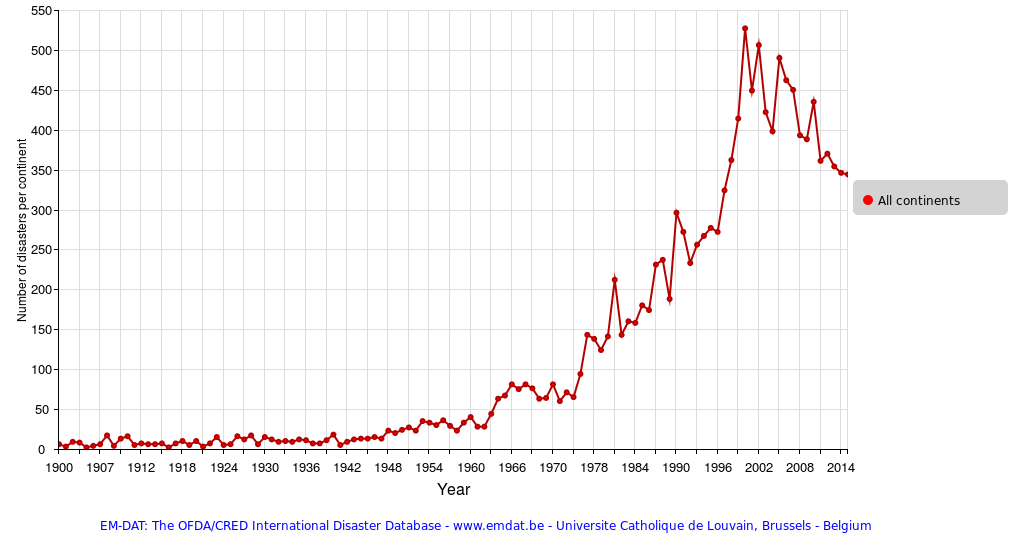
\includegraphics[width=0.65\textwidth]{./figures/catastrofesnaturales.png}
\caption{Número de desastres naturales registrados en el periodo 1900-2015.}
\end{figure}

Con el auge existente en torno a los drones, en la sociedad actual, se abre todo un mundo de posibilidades para la creación de sistemas que sean útiles para la humanidad. Según Sophic Capital y como muestra la \textbf{Figura 2} \cite{cuotamercado} los ingresos totales de las compañías que trabajan con UAVs pueden ascender hasta más de 12000 millones de dólares en el año 2025.


\begin{figure}[htb]
\centering
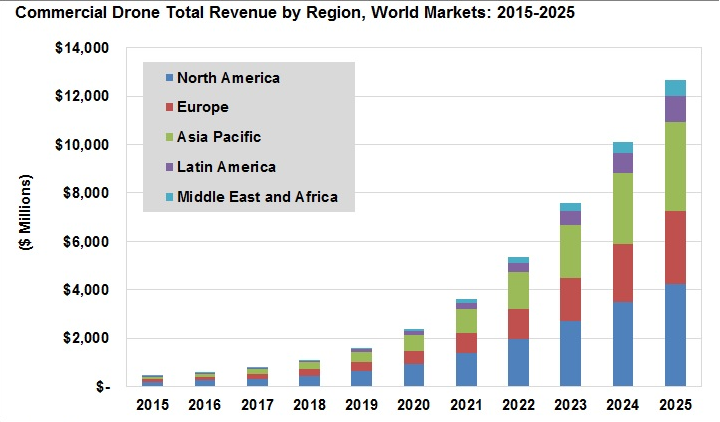
\includegraphics[width=0.60\textwidth]{./figures/DCA-15-chart.png}
\caption{Previsión de ingresos por regiones en el periodo 2015-2025.}
\end{figure} 


\subsection{Motivación}

Estimar el tiempo de actuación en labores de socorro es una tarea compleja, pero los drones pueden desplegarse con rapidez y acortar sustancialmente el tiempo de respuesta y el riesgo de lesiones de los individuos desaparecidos y de los equipos de rescate. En el caso de rescates acuáticos, según la empresa Vodafone \cite{tiempomenor} ``un socorrista tarda el triple del tiempo que un dron necesita para llegar a un bañista en peligro''.

Los UAVs son un aliado perfecto en misiones de búsqueda y rescate puesto que sus limitaciones en condiciones meteorológicas adversas son menores. Aparte de esto, el uso de sensores especializados contribuyen a equipar los UAV de ventajas importantes en la realización de este tipo de operaciones. Sirva como precedente ``la utilización de helicópteros no tripulados franceses Elipse HE 300 durante la actual crisis de la central de Fukushima'' \cite{notripulados}.

Con todo lo anterior, en este TFG se pretende mejorar la productividad de los equipos de rescate, en situaciones de catástrofe, permitiendo rebajar los tiempos de reconocimiento del terreno con la ayuda de una flota de UAVs que se coordinen y comuniquen de forma descentralizada.

El objetivo principal del proyecto es la creación de un sistema que permita monitorizar determinadas zonas, basándose en prioridades, de tal forma que en caso de catástrofe el uso de este software permita reducir costes en cuanto a: i) el tiempo de reconocimiento del territorio afectado por el desastre, ii) el tiempo de rescate de individuos y iii) la exposición al peligro por parte del personal de emergencia.

\begin{figure}[htb]
\centering
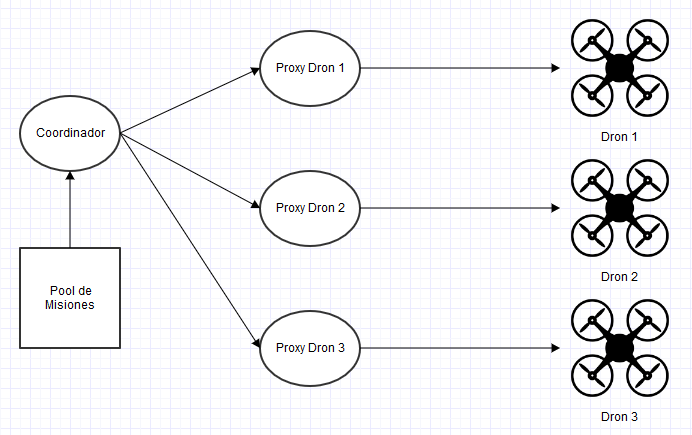
\includegraphics[width=0.8\textwidth]{./figures/dron.png}
\caption{Ejemplo básico del funcionamiento del sistema.}
\end{figure} 

\clearpage
   
\section{TECNOLOGÍA ESPECÍFICA CURSADA POR EL ALUMNO}

\begin{table}[hp]
  \centering
  \caption{Tecnología Específica cursada por el alumno}
  \label{tab:tec-especifica}

  \zebrarows{1}
  \begin{tabular}{p{0.6\textwidth}}
    \textbf{Marcar la tecnología cursada} \\
    \hline
    \quad \enspace Tecnologías de la Información \\
    \checkmark \enspace Computación \\
    \quad \enspace Ingeniería del Software \\
    \quad \enspace Ingeniería de Computadores \\
    \hline
  \end{tabular}
\end{table}

\begin{table}[hp]
  \centering
  \caption{Justificación de las competencias específicas abordadas en el TFG}
  \label{tab:competencias}

  \zebrarows{1}
  \begin{tabular}{p{0.5\linewidth}p{0.5\linewidth}}
    \textbf{Competencia} & \textbf{Justificación} \\
    \hline
   Capacidad para tener un conocimiento profundo de los principios fundamentales y
  modelos de la computación y saberlos aplicar para interpretar, seleccionar, valorar,
  modelar, y crear nuevos conceptos, teorías, usos y desarrollos tecnológicos relacionados
  con la informática. & En este proyecto se pretende desarrollar un sistema en el que diferentes  
UAVs se organicen para poder ser utilizados en situaciones de emergencia. \\
   Capacidad para adquirir, obtener, formalizar y representar el conocimiento humano en
  una forma computable para la resolución de problemas mediante un sistema informático en
  cualquier ámbito de aplicación, particularmente los relacionados con aspectos de
  computación, percepción y actuación en ambientes entornos inteligentes. & Es fundamental modelar el
conocimiento humano para el sistema propuesto, debido a que los drones deben actuar y coordinarse siguiendo las
pautas de los protocolos de actuación establecidos dependiendo de la catástrofe ocurrida. \\
    & \\
    \hline
  \end{tabular}
\end{table}


\section{OBJETIVOS}

Los objetivos que se pretenden conseguir con la realización de este TFG son los siguientes:

\begin{itemize}

\item Desarrollar un sistema adaptativo basado en la coordinación de UAVs o drones para obtener información relevante sobre el entorno afectado por la catástrofe, de forma que se logren los siguientes subobjetivos:

\begin{itemize}
\item Reducir la exposición de agentes humanos al peligro derivado de la propia catástrofe.
\item Minimizar el tiempo empleado en recoger información sobre la zona afectada para el equipo de rescate.
\item Minimizar el daño resultante global.

\end{itemize}

\item Solicitar dispositivos de monitorización bajo demanda cuando sea necesario.

\item Plantear la coordinación entre los UAVs de manera descentralizada para incrementar la robustez del sistema.

\item Identificar diferentes puntos de monitorización, en función a un sistema de prioridades con el objetivo de reunir información en base a la importancia de cada uno de los puntos del entorno monitorizado.

\end {itemize}

\section{MÉTODO Y FASES DE TRABAJO}

El TFG será desarrollado siguiendo un modelo iterativo e incremental.

Dada la complejidad del sistema, lo habitual es que las especificaciones no se desarrollen de una única vez. El proyecto se dividirá en pequeños hitos cuyo desarrollo es una iteración que incrementa la funcionalidad del sistema.

``Una iteración se desarrolla siguiendo el método en cascada, tratando todos los flujos de trabajo fundamentales [...] y concluye con una versión más elaborada del producto.'' \cite{ingsoftware}.

Al comienzo de cada iteración se deben seleccionar y especificar los casos de usos con más relevancia, para a continuación analizar estos casos de uso, diseñarlos, implementarlos mediante componentes y verificar que los componentes satisfagan los casos de uso. Una vez que la iteración cumple con los objetivos se prosigue con la siguiente, creciendo así el sistema de forma incremental al incorporar nuevas funcionalidades en cada ciclo de desarrollo.   

Gracias al uso del modelo iterativo e incremental se reducen los riesgos dada la retroalimentación semanal que existe, en este caso, con David Vallejo como director del TFG. Por otro lado, el desarrollo iterativo e incremental proporciona una mayor flexibilidad a la hora de realizar modificaciones y respecto a la complejidad, dada su división en hitos, jamás debe resultar abrumadora.

La elaboración del proyecto se dividirá en las siguientes partes:

\subsection{Estado del Arte}

En esta primera etapa se lleva a cabo una prospección de los sistemas y artículos que se han realizado hasta la fecha y que se correspondan con la utilización de UAVs en situaciones de emergencia. Asimismo, se analizarán  las tecnologías más importantes para el desarrollo e implementación del sistema adaptativo.

\subsection{Análisis y Diseño}

La documentación continuará con un análisis de requisitos que permita comprender la naturaleza del sistema, su función, comportamiento e interconexión \cite{pressman}. Después, en la fase de diseño se establecen las estructuras de datos, la arquitectura del software, y una representación de la interfaz y el algoritmo sobre los cuales se trabajarán en fases posteriores. ``El proceso de diseño traduce requisitos en una representación de software'' \cite{pressman}

\subsection{Implementación y Pruebas}

Esta actividad tratará de traducir el diseño a un lenguaje de programación legible por la computadora, Python en este caso. Una vez que se haya implementado el código, las pruebas del software se centrarán en asegurarse que todas las sentencias se han comprobado y en realizar las prueba para la detección de errores \cite{pressman}.

\subsection{Análisis de Resultados}

Se efectuará una evaluación en cada iteración de las nuevas funcionalidades incorporadas al proyecto.

\section{MEDIOS QUE SE PRETENDEN UTILIZAR}

\subsection{Medios Hardware}
Los medios hardware necesarios para el desarrollo del proyecto son:

\begin{itemize}
\item \textbf{Computador Packard Bell EN-TS44HR}: para el desarrollo del Trabajo Fin de Grado.
\item \textbf{Quadcopter 3DR IRIS+\footnote{https://store.3dr.com/products/IRIS}}: equipo para el despliegue final del sistema propuesto. 3DR IRIS+ hace uso de:

\begin{itemize}
\item \textbf{Piloto automático Pixhawk\footnote{http://copter.ardupilot.com/wiki/common-pixhawk-overview/}}: es un piloto automático de alto rendimiento para vehículos de ala fija, múltiples rotores, helicópteros, coches, barcos y cualquier otra plataforma robótica que se puede mover.
\item \textbf{GoPro HERO 3+\footnote{https://es.gopro.com/support/articles/hero3plus-camera-comparison}}: permite la visualización en primera persona de imágenes en directo, así como la grabación de las mismas.
\item \textbf{Tarot T-2D Gimbal\footnote{https://store.3dr.com/products/tarot-t-2d-brushless-gimbal-kit}}: asegura obtener imágenes estables y claras desde el 3DR IRIS+.
\item \textbf{SiK Telemetry Radio\footnote{http://copter.ardupilot.com/wiki/common-3dr-radio-version-2/}}: es una de las maneras más fáciles de configurar una conexión de telemetría entre el Pixhawk y una estación terrestre.
\item \textbf{Módulo GPS\footnote{http://copter.ardupilot.com/wiki/common-installing-3dr-ublox-gps-compass-module/}}: utiliza el sistema de posicionamiento global para determinar y realizar un seguimiento de su ubicación precisa.
\end{itemize}

\end{itemize}
\subsection{Medios Software}
Los medios software necesarios para el desarrollo del proyecto son:

\begin{itemize}
\item \textbf{GNU/Linux Ubuntu\footnote{http://www.ubuntu.com/}}.
\item \textbf{Git 1.9.1\footnote{https://git-scm.com/}}: para alojar proyectos, en un repositorio online de GitHub, haciendo uso del sistema de control de versiones.
\item \textbf{APM Planner 2.0\footnote{http://planner2.ardupilot.com/}}: es una estación terrestre de código abierto para pilotos automáticos basados en MAVlink, incluyendo Pixhawk. Puede ejecutarse en Windows, Mac OS X y Linux.
\item \textbf{Software in the Loop (SITL)\footnote{http://dev.ardupilot.com/wiki/sitl-simulator-software-in-the-loop/}}: permite poner a prueba el comportamiento del código sin necesidad de hardware. Para el uso de SITL es necesario instalar:
\begin{itemize}
\item \textbf{ArduPilot\footnote{http://ardupilot.com/}}: es un piloto automático portátil que puede funcionar en una amplia variedad de plataformas. El computador es simplemente otra plataforma en la que ArduPilot se puede ejecutar.
\item \textbf{MAVProxy\footnote{http://dronecode.github.io/MAVProxy/html/index.html}}: es una estación de control de tierra minimalista, portátil y extensible para cualquier UAV que soporte el protocolo MAVLink.
\item \textbf{MAVLink\footnote{http://qgroundcontrol.org/mavlink/start}}: protocolo para la comunicación entre la estación de tierra, controlador de vuelo y algunos periféricos.
\end {itemize}
\item \textbf{Python\footnote{https://www.python.org/}}: el proyecto será desarrollado haciendo uso del lenguaje de programación Python, ya que se dispone de un kit de desarrollo (o SDK) en este lenguaje que facilitará la implementación considerablemente:
\begin {itemize}
\item \textbf{Dronekit-Python\footnote{http://python.dronekit.io/}}: ayuda a crear aplicaciones potentes para vehículos aéreos no tripulados. Dichas aplicaciones se ejecutan en un ordenador y aumentan la funcionalidad del piloto automático mediante la realización de tareas que son computacionalmente intensivas y requieren un enlace de baja latencia.
\end{itemize}
\item \textbf{ZeroC ICE\footnote{https://zeroc.com/products/ice}}: con el que se plantea la parte de comunicación y del servidor. 
\item \textbf{LaTeX\footnote{http://www.latex-project.org/}}: usado para la creación de documentos escritos que presenten una calidad superior.
\item \textbf{GNU Emacs\footnote{https://www.gnu.org/software/emacs/}}: editor de texto utilizado para la creación de la documentación en LaTeX y del código fuente.
\end{itemize}

\bibliographystyle{acm}
\singlespacing
\bibliography{main}

\end{document}


% Local Variables:
% coding: utf-8
% mode: flyspell
% ispell-local-dictionary: "castellano8"
% mode: latex
% End:
